% Created by tikzDevice version 0.12.3.1 on 2023-04-12 14:29:24
% !TEX encoding = UTF-8 Unicode
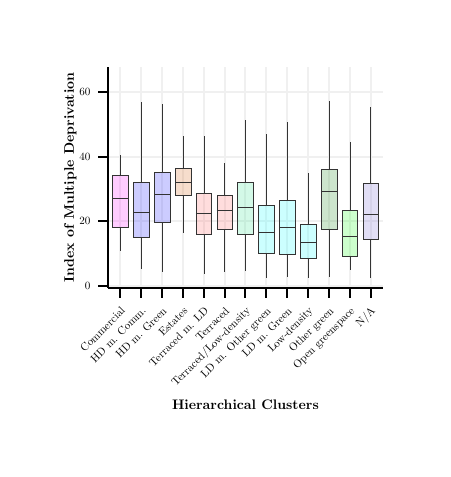
\begin{tikzpicture}[x=1pt,y=1pt]
\definecolor{fillColor}{RGB}{255,255,255}
\path[use as bounding box,fill=fillColor,fill opacity=0.00] (0,0) rectangle (142.64,152.15);
\begin{scope}
\path[clip] (  0.00,  0.00) rectangle (142.64,152.15);
\definecolor{fillColor}{RGB}{255,255,255}

\path[fill=fillColor] (  0.00,  0.00) rectangle (142.64,152.15);
\end{scope}
\begin{scope}
\path[clip] ( 28.95, 58.04) rectangle (128.41,137.92);
\definecolor{fillColor}{RGB}{255,255,255}

\path[fill=fillColor] ( 28.95, 58.04) rectangle (128.41,137.92);
\definecolor{drawColor}{gray}{0.94}

\path[draw=drawColor,line width= 0.7pt,line join=round] ( 28.95, 58.96) --
	(128.41, 58.96);

\path[draw=drawColor,line width= 0.7pt,line join=round] ( 28.95, 82.25) --
	(128.41, 82.25);

\path[draw=drawColor,line width= 0.7pt,line join=round] ( 28.95,105.55) --
	(128.41,105.55);

\path[draw=drawColor,line width= 0.7pt,line join=round] ( 28.95,128.84) --
	(128.41,128.84);

\path[draw=drawColor,line width= 0.7pt,line join=round] ( 33.47, 58.04) --
	( 33.47,137.92);

\path[draw=drawColor,line width= 0.7pt,line join=round] ( 41.00, 58.04) --
	( 41.00,137.92);

\path[draw=drawColor,line width= 0.7pt,line join=round] ( 48.54, 58.04) --
	( 48.54,137.92);

\path[draw=drawColor,line width= 0.7pt,line join=round] ( 56.07, 58.04) --
	( 56.07,137.92);

\path[draw=drawColor,line width= 0.7pt,line join=round] ( 63.61, 58.04) --
	( 63.61,137.92);

\path[draw=drawColor,line width= 0.7pt,line join=round] ( 71.14, 58.04) --
	( 71.14,137.92);

\path[draw=drawColor,line width= 0.7pt,line join=round] ( 78.68, 58.04) --
	( 78.68,137.92);

\path[draw=drawColor,line width= 0.7pt,line join=round] ( 86.21, 58.04) --
	( 86.21,137.92);

\path[draw=drawColor,line width= 0.7pt,line join=round] ( 93.75, 58.04) --
	( 93.75,137.92);

\path[draw=drawColor,line width= 0.7pt,line join=round] (101.29, 58.04) --
	(101.29,137.92);

\path[draw=drawColor,line width= 0.7pt,line join=round] (108.82, 58.04) --
	(108.82,137.92);

\path[draw=drawColor,line width= 0.7pt,line join=round] (116.36, 58.04) --
	(116.36,137.92);

\path[draw=drawColor,line width= 0.7pt,line join=round] (123.89, 58.04) --
	(123.89,137.92);
\definecolor{drawColor}{gray}{0.20}

\path[draw=drawColor,line width= 0.1pt,line join=round] ( 41.00, 96.38) -- ( 41.00,125.46);

\path[draw=drawColor,line width= 0.1pt,line join=round] ( 41.00, 76.30) -- ( 41.00, 64.95);
\definecolor{fillColor}{RGB}{0,0,255}

\path[draw=drawColor,line width= 0.1pt,fill=fillColor,fill opacity=0.20] ( 38.18, 96.38) --
	( 38.18, 76.30) --
	( 43.83, 76.30) --
	( 43.83, 96.38) --
	( 38.18, 96.38) --
	cycle;

\path[draw=drawColor,line width= 0.1pt] ( 38.18, 85.58) -- ( 43.83, 85.58);

\path[draw=drawColor,line width= 0.1pt,line join=round] ( 33.47, 98.85) -- ( 33.47,106.18);

\path[draw=drawColor,line width= 0.1pt,line join=round] ( 33.47, 80.15) -- ( 33.47, 71.61);
\definecolor{fillColor}{RGB}{255,0,255}

\path[draw=drawColor,line width= 0.1pt,fill=fillColor,fill opacity=0.20] ( 30.64, 98.85) --
	( 30.64, 80.15) --
	( 36.29, 80.15) --
	( 36.29, 98.85) --
	( 30.64, 98.85) --
	cycle;

\path[draw=drawColor,line width= 0.1pt] ( 30.64, 90.59) -- ( 36.29, 90.59);

\path[draw=drawColor,line width= 0.1pt,line join=round] ( 86.21, 87.95) -- ( 86.21,113.57);

\path[draw=drawColor,line width= 0.1pt,line join=round] ( 86.21, 70.74) -- ( 86.21, 61.68);
\definecolor{fillColor}{RGB}{0,255,255}

\path[draw=drawColor,line width= 0.1pt,fill=fillColor,fill opacity=0.20] ( 83.39, 87.95) --
	( 83.39, 70.74) --
	( 89.04, 70.74) --
	( 89.04, 87.95) --
	( 83.39, 87.95) --
	cycle;

\path[draw=drawColor,line width= 0.1pt] ( 83.39, 78.23) -- ( 89.04, 78.23);

\path[draw=drawColor,line width= 0.1pt,line join=round] ( 93.75, 89.96) -- ( 93.75,118.02);

\path[draw=drawColor,line width= 0.1pt,line join=round] ( 93.75, 70.38) -- ( 93.75, 61.95);

\path[draw=drawColor,line width= 0.1pt,fill=fillColor,fill opacity=0.20] ( 90.92, 89.96) --
	( 90.92, 70.38) --
	( 96.58, 70.38) --
	( 96.58, 89.96) --
	( 90.92, 89.96) --
	cycle;

\path[draw=drawColor,line width= 0.1pt] ( 90.92, 80.16) -- ( 96.58, 80.16);

\path[draw=drawColor,line width= 0.1pt,line join=round] (108.82,101.11) -- (108.82,125.63);

\path[draw=drawColor,line width= 0.1pt,line join=round] (108.82, 79.49) -- (108.82, 62.16);
\definecolor{fillColor}{RGB}{0,128,0}

\path[draw=drawColor,line width= 0.1pt,fill=fillColor,fill opacity=0.20] (105.99,101.11) --
	(105.99, 79.49) --
	(111.65, 79.49) --
	(111.65,101.11) --
	(105.99,101.11) --
	cycle;

\path[draw=drawColor,line width= 0.1pt] (105.99, 93.01) -- (111.65, 93.01);

\path[draw=drawColor,line width= 0.1pt,line join=round] ( 63.61, 92.26) -- ( 63.61,113.05);

\path[draw=drawColor,line width= 0.1pt,line join=round] ( 63.61, 77.65) -- ( 63.61, 63.12);
\definecolor{fillColor}{RGB}{255,85,85}

\path[draw=drawColor,line width= 0.1pt,fill=fillColor,fill opacity=0.20] ( 60.78, 92.26) --
	( 60.78, 77.65) --
	( 66.44, 77.65) --
	( 66.44, 92.26) --
	( 60.78, 92.26) --
	cycle;

\path[draw=drawColor,line width= 0.1pt] ( 60.78, 85.23) -- ( 66.44, 85.23);

\path[draw=drawColor,line width= 0.1pt,line join=round] ( 48.54, 99.97) -- ( 48.54,124.49);

\path[draw=drawColor,line width= 0.1pt,line join=round] ( 48.54, 81.90) -- ( 48.54, 63.99);
\definecolor{fillColor}{RGB}{0,0,255}

\path[draw=drawColor,line width= 0.1pt,fill=fillColor,fill opacity=0.20] ( 45.71, 99.97) --
	( 45.71, 81.90) --
	( 51.36, 81.90) --
	( 51.36, 99.97) --
	( 45.71, 99.97) --
	cycle;

\path[draw=drawColor,line width= 0.1pt] ( 45.71, 92.13) -- ( 51.36, 92.13);

\path[draw=drawColor,line width= 0.1pt,line join=round] ( 71.14, 91.53) -- ( 71.14,103.08);

\path[draw=drawColor,line width= 0.1pt,line join=round] ( 71.14, 79.39) -- ( 71.14, 64.04);
\definecolor{fillColor}{RGB}{255,85,85}

\path[draw=drawColor,line width= 0.1pt,fill=fillColor,fill opacity=0.20] ( 68.32, 91.53) --
	( 68.32, 79.39) --
	( 73.97, 79.39) --
	( 73.97, 91.53) --
	( 68.32, 91.53) --
	cycle;

\path[draw=drawColor,line width= 0.1pt] ( 68.32, 86.15) -- ( 73.97, 86.15);

\path[draw=drawColor,line width= 0.1pt,line join=round] (101.29, 81.17) -- (101.29, 99.67);

\path[draw=drawColor,line width= 0.1pt,line join=round] (101.29, 68.76) -- (101.29, 61.67);
\definecolor{fillColor}{RGB}{0,255,255}

\path[draw=drawColor,line width= 0.1pt,fill=fillColor,fill opacity=0.20] ( 98.46, 81.17) --
	( 98.46, 68.76) --
	(104.11, 68.76) --
	(104.11, 81.17) --
	( 98.46, 81.17) --
	cycle;

\path[draw=drawColor,line width= 0.1pt] ( 98.46, 74.68) -- (104.11, 74.68);

\path[draw=drawColor,line width= 0.1pt,line join=round] ( 78.68, 96.26) -- ( 78.68,118.85);

\path[draw=drawColor,line width= 0.1pt,line join=round] ( 78.68, 77.42) -- ( 78.68, 64.18);
\definecolor{fillColor}{RGB}{37,229,137}

\path[draw=drawColor,line width= 0.1pt,fill=fillColor,fill opacity=0.20] ( 75.85, 96.26) --
	( 75.85, 77.42) --
	( 81.51, 77.42) --
	( 81.51, 96.26) --
	( 75.85, 96.26) --
	cycle;

\path[draw=drawColor,line width= 0.1pt] ( 75.85, 87.36) -- ( 81.51, 87.36);

\path[draw=drawColor,line width= 0.1pt,line join=round] (116.36, 86.20) -- (116.36,110.98);

\path[draw=drawColor,line width= 0.1pt,line join=round] (116.36, 69.68) -- (116.36, 64.43);
\definecolor{fillColor}{RGB}{0,255,0}

\path[draw=drawColor,line width= 0.1pt,fill=fillColor,fill opacity=0.20] (113.53, 86.20) --
	(113.53, 69.68) --
	(119.18, 69.68) --
	(119.18, 86.20) --
	(113.53, 86.20) --
	cycle;

\path[draw=drawColor,line width= 0.1pt] (113.53, 76.86) -- (119.18, 76.86);

\path[draw=drawColor,line width= 0.1pt,line join=round] ( 56.07,101.28) -- ( 56.07,113.07);

\path[draw=drawColor,line width= 0.1pt,line join=round] ( 56.07, 91.52) -- ( 56.07, 77.97);
\definecolor{fillColor}{RGB}{212,85,0}

\path[draw=drawColor,line width= 0.1pt,fill=fillColor,fill opacity=0.20] ( 53.25,101.28) --
	( 53.25, 91.52) --
	( 58.90, 91.52) --
	( 58.90,101.28) --
	( 53.25,101.28) --
	cycle;

\path[draw=drawColor,line width= 0.1pt] ( 53.25, 96.40) -- ( 58.90, 96.40);

\path[draw=drawColor,line width= 0.1pt,line join=round] (123.89, 95.95) -- (123.89,123.50);

\path[draw=drawColor,line width= 0.1pt,line join=round] (123.89, 75.56) -- (123.89, 61.82);
\definecolor{fillColor}{RGB}{106,90,205}

\path[draw=drawColor,line width= 0.1pt,fill=fillColor,fill opacity=0.20] (121.07, 95.95) --
	(121.07, 75.56) --
	(126.72, 75.56) --
	(126.72, 95.95) --
	(121.07, 95.95) --
	cycle;

\path[draw=drawColor,line width= 0.1pt] (121.07, 84.95) -- (126.72, 84.95);

\path[] ( 28.95, 58.04) rectangle (128.41,137.92);
\end{scope}
\begin{scope}
\path[clip] (  0.00,  0.00) rectangle (142.64,152.15);
\definecolor{drawColor}{RGB}{0,0,0}

\path[draw=drawColor,line width= 0.7pt,line join=round] ( 28.95, 58.04) --
	( 28.95,137.92);
\end{scope}
\begin{scope}
\path[clip] (  0.00,  0.00) rectangle (142.64,152.15);
\definecolor{drawColor}{RGB}{0,0,0}

\node[text=drawColor,anchor=base east,inner sep=0pt, outer sep=0pt, scale=  0.40] at ( 22.65, 57.58) {0};

\node[text=drawColor,anchor=base east,inner sep=0pt, outer sep=0pt, scale=  0.40] at ( 22.65, 80.88) {20};

\node[text=drawColor,anchor=base east,inner sep=0pt, outer sep=0pt, scale=  0.40] at ( 22.65,104.17) {40};

\node[text=drawColor,anchor=base east,inner sep=0pt, outer sep=0pt, scale=  0.40] at ( 22.65,127.47) {60};
\end{scope}
\begin{scope}
\path[clip] (  0.00,  0.00) rectangle (142.64,152.15);
\definecolor{drawColor}{RGB}{0,0,0}

\path[draw=drawColor,line width= 0.7pt,line join=round] ( 25.45, 58.96) --
	( 28.95, 58.96);

\path[draw=drawColor,line width= 0.7pt,line join=round] ( 25.45, 82.25) --
	( 28.95, 82.25);

\path[draw=drawColor,line width= 0.7pt,line join=round] ( 25.45,105.55) --
	( 28.95,105.55);

\path[draw=drawColor,line width= 0.7pt,line join=round] ( 25.45,128.84) --
	( 28.95,128.84);
\end{scope}
\begin{scope}
\path[clip] (  0.00,  0.00) rectangle (142.64,152.15);
\definecolor{drawColor}{RGB}{0,0,0}

\path[draw=drawColor,line width= 0.7pt,line join=round] ( 28.95, 58.04) --
	(128.41, 58.04);
\end{scope}
\begin{scope}
\path[clip] (  0.00,  0.00) rectangle (142.64,152.15);
\definecolor{drawColor}{RGB}{0,0,0}

\path[draw=drawColor,line width= 0.7pt,line join=round] ( 33.47, 54.54) --
	( 33.47, 58.04);

\path[draw=drawColor,line width= 0.7pt,line join=round] ( 41.00, 54.54) --
	( 41.00, 58.04);

\path[draw=drawColor,line width= 0.7pt,line join=round] ( 48.54, 54.54) --
	( 48.54, 58.04);

\path[draw=drawColor,line width= 0.7pt,line join=round] ( 56.07, 54.54) --
	( 56.07, 58.04);

\path[draw=drawColor,line width= 0.7pt,line join=round] ( 63.61, 54.54) --
	( 63.61, 58.04);

\path[draw=drawColor,line width= 0.7pt,line join=round] ( 71.14, 54.54) --
	( 71.14, 58.04);

\path[draw=drawColor,line width= 0.7pt,line join=round] ( 78.68, 54.54) --
	( 78.68, 58.04);

\path[draw=drawColor,line width= 0.7pt,line join=round] ( 86.21, 54.54) --
	( 86.21, 58.04);

\path[draw=drawColor,line width= 0.7pt,line join=round] ( 93.75, 54.54) --
	( 93.75, 58.04);

\path[draw=drawColor,line width= 0.7pt,line join=round] (101.29, 54.54) --
	(101.29, 58.04);

\path[draw=drawColor,line width= 0.7pt,line join=round] (108.82, 54.54) --
	(108.82, 58.04);

\path[draw=drawColor,line width= 0.7pt,line join=round] (116.36, 54.54) --
	(116.36, 58.04);

\path[draw=drawColor,line width= 0.7pt,line join=round] (123.89, 54.54) --
	(123.89, 58.04);
\end{scope}
\begin{scope}
\path[clip] (  0.00,  0.00) rectangle (142.64,152.15);
\definecolor{drawColor}{RGB}{0,0,0}

\node[text=drawColor,rotate= 45.00,anchor=base east,inner sep=0pt, outer sep=0pt, scale=  0.40] at ( 35.40, 49.51) {Commercial};

\node[text=drawColor,rotate= 45.00,anchor=base east,inner sep=0pt, outer sep=0pt, scale=  0.40] at ( 42.93, 49.51) {HD m. Comm.};

\node[text=drawColor,rotate= 45.00,anchor=base east,inner sep=0pt, outer sep=0pt, scale=  0.40] at ( 50.47, 49.51) {HD m. Green};

\node[text=drawColor,rotate= 45.00,anchor=base east,inner sep=0pt, outer sep=0pt, scale=  0.40] at ( 58.00, 49.51) {Estates};

\node[text=drawColor,rotate= 45.00,anchor=base east,inner sep=0pt, outer sep=0pt, scale=  0.40] at ( 65.54, 49.51) {Terraced m. LD};

\node[text=drawColor,rotate= 45.00,anchor=base east,inner sep=0pt, outer sep=0pt, scale=  0.40] at ( 73.07, 49.51) {Terraced};

\node[text=drawColor,rotate= 45.00,anchor=base east,inner sep=0pt, outer sep=0pt, scale=  0.40] at ( 80.61, 49.51) {Terraced/Low-density};

\node[text=drawColor,rotate= 45.00,anchor=base east,inner sep=0pt, outer sep=0pt, scale=  0.40] at ( 88.14, 49.51) {LD m. Other green};

\node[text=drawColor,rotate= 45.00,anchor=base east,inner sep=0pt, outer sep=0pt, scale=  0.40] at ( 95.68, 49.51) {LD m. Green};

\node[text=drawColor,rotate= 45.00,anchor=base east,inner sep=0pt, outer sep=0pt, scale=  0.40] at (103.21, 49.51) {Low-density};

\node[text=drawColor,rotate= 45.00,anchor=base east,inner sep=0pt, outer sep=0pt, scale=  0.40] at (110.75, 49.51) {Other green};

\node[text=drawColor,rotate= 45.00,anchor=base east,inner sep=0pt, outer sep=0pt, scale=  0.40] at (118.28, 49.51) {Open greenspace};

\node[text=drawColor,rotate= 45.00,anchor=base east,inner sep=0pt, outer sep=0pt, scale=  0.40] at (125.82, 49.51) {N/A};
\end{scope}
\begin{scope}
\path[clip] (  0.00,  0.00) rectangle (142.64,152.15);
\definecolor{drawColor}{RGB}{0,0,0}

\node[text=drawColor,anchor=base,inner sep=0pt, outer sep=0pt, scale=  0.50] at ( 78.68, 14.03) {\bfseries Hierarchical Clusters};
\end{scope}
\begin{scope}
\path[clip] (  0.00,  0.00) rectangle (142.64,152.15);
\definecolor{drawColor}{RGB}{0,0,0}

\node[text=drawColor,rotate= 90.00,anchor=base,inner sep=0pt, outer sep=0pt, scale=  0.50] at ( 16.70, 97.98) {\bfseries Index of Multiple Deprivation};
\end{scope}
\end{tikzpicture}
